%==============================================================================
% AIP Advances Highlight Image (Native Coordinates - No Scaling/Transforms)
% Canvas size: 8.0139 in × 6.2739 in (exact)
%==============================================================================

\documentclass{article}

\usepackage[
    paperwidth=8.0139in,
    paperheight=6.2739in,
    margin=0in
]{geometry}

\usepackage[T1]{fontenc}
\usepackage[utf8]{inputenc}
\usepackage{newtxtext,newtxmath}
\usepackage{tikz}
\usetikzlibrary{arrows.meta,calc,positioning}

\pagestyle{empty}
\begin{document}
    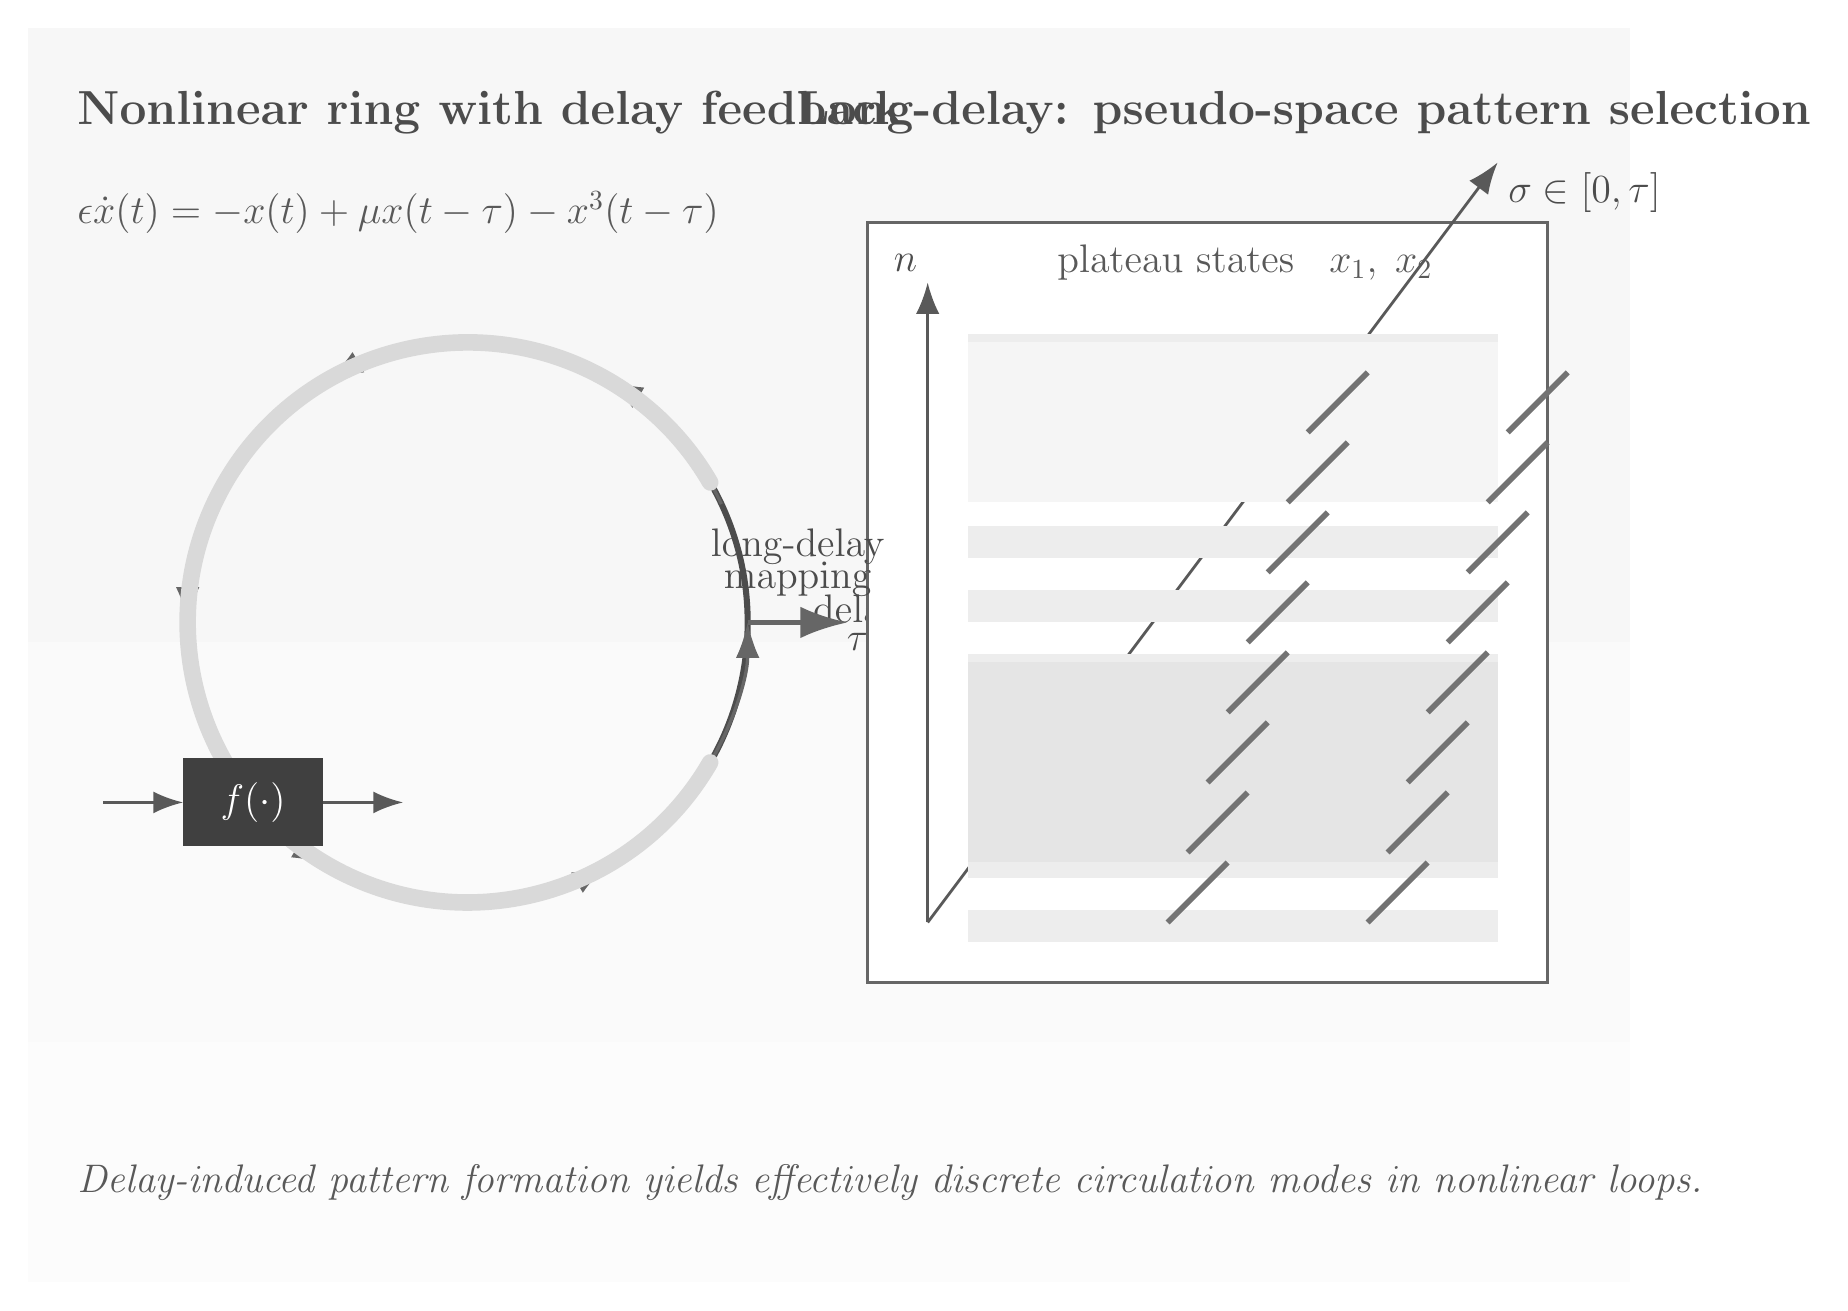
\begin{tikzpicture}[x=1in,y=1in]

        % 1. Canvas Background
        \fill[black!2] (0,0) rectangle (8.0139,6.2739);
        \fill[black!3] (0,3.2) rectangle (8.0139,6.2739);
        \fill[black!1] (0,0) rectangle (8.0139,1.2);

        %-----------------------------------------------------------------------
        % LEFT PANEL: Nonlinear ring + delay
        %-----------------------------------------------------------------------
        \coordinate (C) at (2.2,3.3);
        \def\R{1.4}

        \draw[line width=2.2pt, black!70] (C) circle (\R);

        \foreach \ang in {25,85,145,205,265,325} {
            \draw[-{Latex[length=4.5mm,width=3.0mm]}, line width=1.2pt, black!60]
            ($(C)+(\ang:\R)$) arc[start angle=\ang, end angle=\ang+35, radius=\R];
        }

        \draw[line width=6pt, black!15, line cap=round]
        ($(C)+(330:\R)$) arc[start angle=330, end angle=30, radius=\R];

        % Text label now uses standard positioning, no transforms
        \node[align=center, text=black!70] at ($(C)+(0:\R+0.55)$)
            {\Large delay\\[-2pt]\Large $\tau$};

        \coordinate (NL) at ($(C)+(220:\R)$);
        \fill[black!75] ($(NL)+(-0.35,-0.22)$) rectangle ($(NL)+(0.35,0.22)$);
        \node[text=white] at (NL) {\Large $f(\cdot)$};

        \draw[-{Latex[length=3.8mm,width=2.8mm]}, line width=1.0pt, black!65]
        ($(NL)+(-0.75,0)$) -- ($(NL)+(-0.35,0)$);
        \draw[-{Latex[length=3.8mm,width=2.8mm]}, line width=1.0pt, black!65]
        ($(NL)+(0.35,0)$) -- ($(NL)+(0.75,0)$);

        \node[anchor=west, text=black!70] at (0.2,5.85)
            {\LARGE \textbf{Nonlinear ring with delay feedback}};
        \node[anchor=west, text=black!65] at (0.2,5.35)
            {\Large $\epsilon \dot{x}(t) = -x(t) + \mu x(t-\tau) - x^3(t-\tau)$};

        %-----------------------------------------------------------------------
        % RIGHT PANEL: Pseudo-space grid
        %-----------------------------------------------------------------------
        \coordinate (PBL) at (4.2,1.5);
        \coordinate (PTR) at (7.6,5.3);

        \fill[white] (PBL) rectangle (PTR);
        \draw[line width=1.2pt, black!60] (PBL) rectangle (PTR);

        \draw[-{Latex[length=4mm,width=3mm]}, line width=1.0pt, black!65]
        ($(PBL)+(0.3,0.3)$) -- ($(PTR)+(-0.25,0.3)$)
        node[below right, text=black!70] {\Large $\sigma \in [0,\tau]$};
        \draw[-{Latex[length=4mm,width=3mm]}, line width=1.0pt, black!65]
        ($(PBL)+(0.3,0.3)$) -- ($(PBL)+(0.3,3.5)$)
        node[above left, text=black!70] {\Large $n$};

        % Pattern fill adjusted to new coordinates
        \foreach \k in {0,...,9} {
            \pgfmathsetmacro{\yyA}{1.7 + 0.32*\k}
            \pgfmathsetmacro{\yyB}{\yyA + 0.16}
            \fill[black!7]
            ($(PBL)+(0.5,\yyA-1.5)$) rectangle ($(PTR)+(-0.25,\yyB-5.3)$);
        }

        \fill[black!10] ($(PBL)+(0.5,0.6)$) rectangle ($(PTR)+(-0.25,-2.2)$);
        \fill[black!4]  ($(PBL)+(0.5,2.4)$) rectangle ($(PTR)+(-0.25,-0.6)$);

        \foreach \m in {0,...,7} {
            \pgfmathsetmacro{\yy}{1.8 + 0.35*\m}
            \pgfmathsetmacro{\shift}{0.1*\m}
            \draw[line width=2.0pt, black!55]
            ($(PBL)+(1.5+\shift,\yy-1.5)$) -- ($(PBL)+(1.8+\shift,\yy-1.2)$);
            \draw[line width=2.0pt, black!55]
            ($(PBL)+(2.5+\shift,\yy-1.5)$) -- ($(PBL)+(2.8+\shift,\yy-1.2)$);
        }

        \node[anchor=west, text=black!65] at ($(PTR)+(-2.5,-0.2)$)
            {\Large plateau states $\;\;x_1,\;x_2$};

        % Shifted left to ensure text strictly fits within 8.0139in width
        \node[anchor=west, text=black!70] at (3.8,5.85)
            {\LARGE \textbf{Long-delay: pseudo-space pattern selection}};

        %-----------------------------------------------------------------------
        % CONNECTOR
        %-----------------------------------------------------------------------
        \draw[-{Latex[length=6mm,width=4mm]}, line width=1.6pt, black!60]
        (3.6,3.3) -- (4.1,3.3);

        \node[text=black!70, align=center] at (3.85,3.6)
            {\Large long-delay\\[-2pt]\Large mapping};

        %-----------------------------------------------------------------------
        % FOOTER
        %-----------------------------------------------------------------------
        \node[anchor=west, text=black!65] at (0.2,0.5)
            {\Large \textit{Delay-induced pattern formation yields effectively discrete circulation modes in nonlinear loops.}};

    \end{tikzpicture}
\end{document}